\subsection{PS/2 Port}

The {\it \systemNameFull} includes two PS/2 ports that can be connected to a standard PS/2
keyboard or mouse. The port includes a 256-byte FIFO that stores data received from a PS/2
device.  The programming interface for the PS/2 port consists of two registers, 
as illustrated in Figure \ref{fig:PS2_port}. The {\it PS2\_Data} register is both readable
and writable. When bit 15, {\it RVALID}, is 1, reading from this register provides the data 
at the head of the FIFO in the
{\it Data} field, and the number of entries in the FIFO (including this read) in the 
{\it RAVAIL} field. When {\it RVALID} is 1, reading from the {\it PS2\_Data} register
decrements this field by 1. Writing to the {\it PS2\_Data} register can be used to send a
command in the {\it Data} field to the PS/2 device.

The {\it PS2\_Control} register can be used to enable interrupts from the PS/2 port by
setting the {\it RE} field to the value 1. When this field is set, then the PS/2 port
generates an interrupt when {\it RAVAIL} $>$ 0. While the interrupt is pending the
field {\it RI} will be set to 1, and it can be cleared by emptying the PS/2 port FIFO. The
{\it CE} field in the {\it PS2\_Control} register is used to indicate that an error
occurred when sending a command to a PS/2 device.

\begin{figure}[h!]
   \begin{center}
       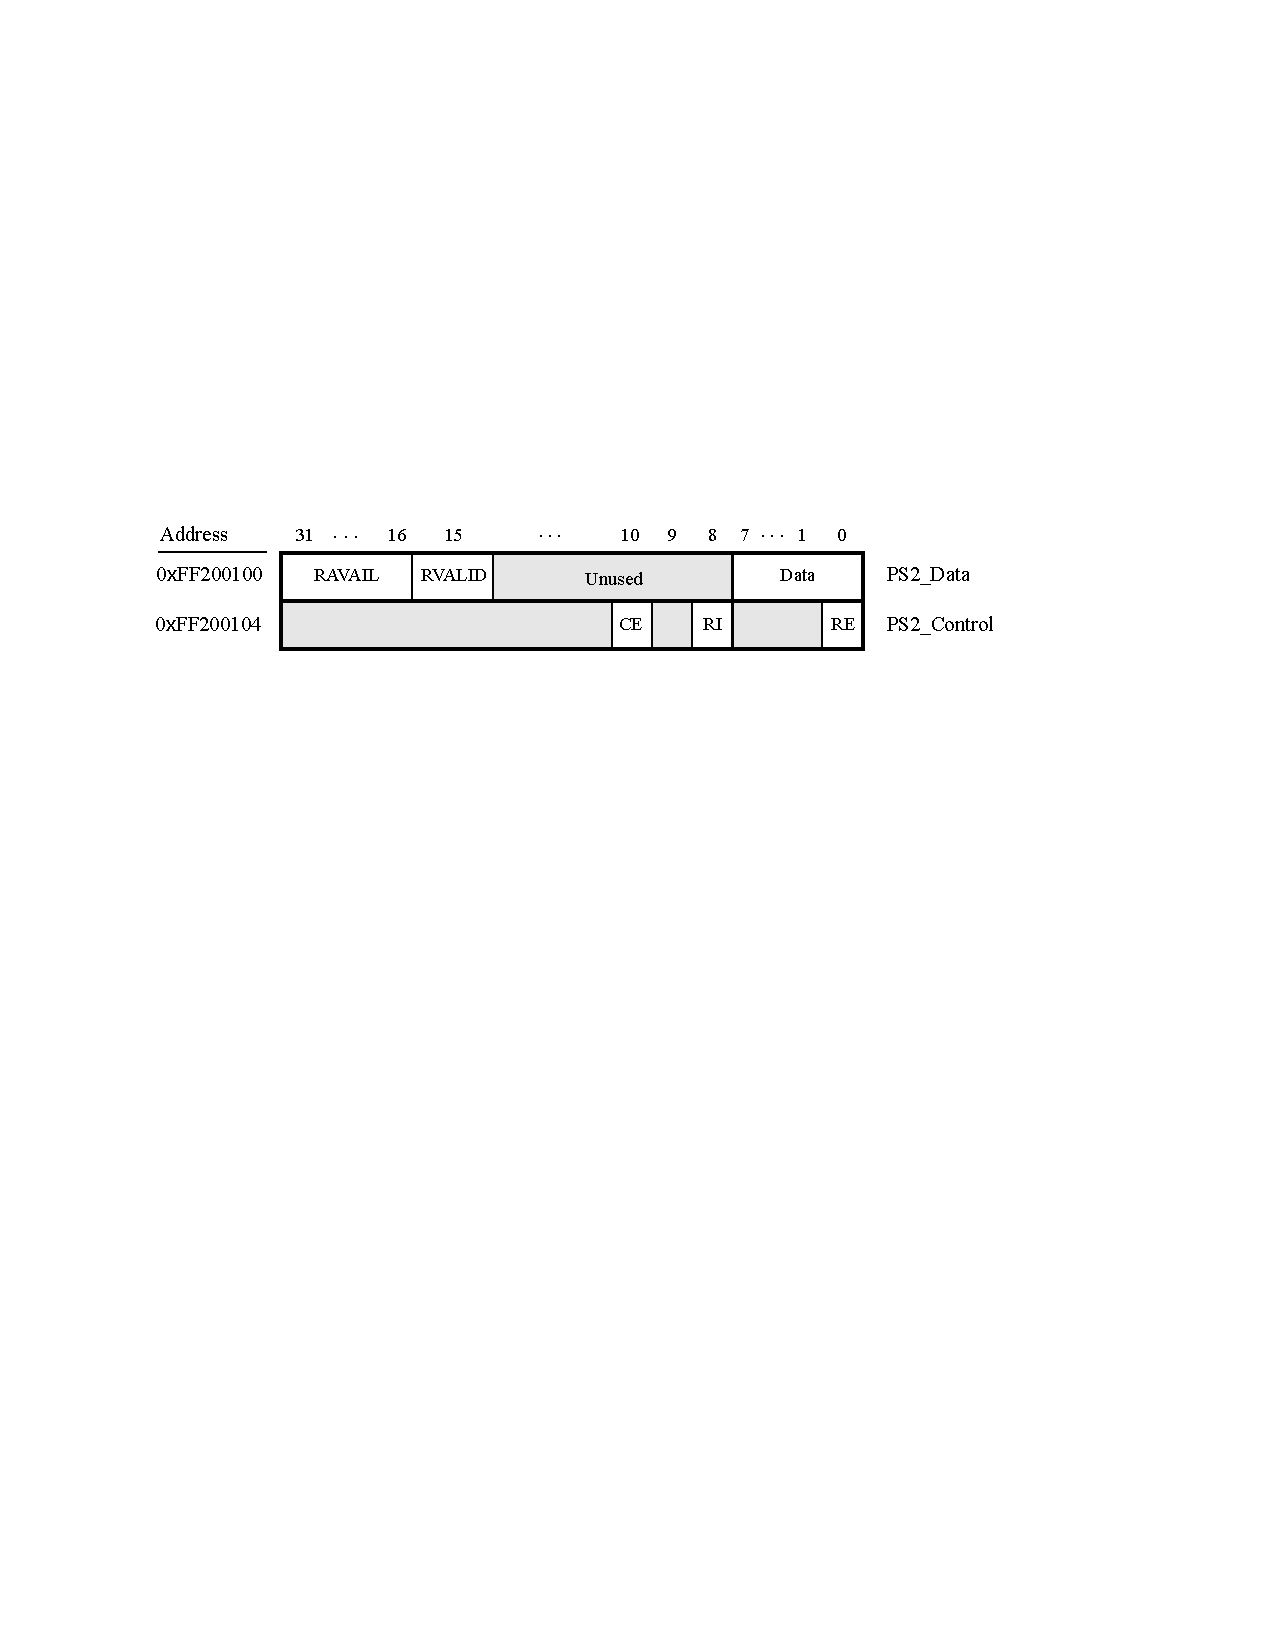
\includegraphics{../../../common/figs/Media_FPGA_PS2.pdf}
   \end{center}
   \caption{PS/2 port registers.}
	\label{fig:PS2_port}
\end{figure}

A fragment of C code that uses the PS/2 port is given in Listing \ref{lst:PS2_C}.  
This code reads the content of the {\it Data} register, and saves data when it is
available.  If the code is used continually in a loop, then it
stores the last three bytes of data received from the
PS/2 port in the variables {\it byte}$_1$, {\it byte}$_2$, and {\it byte}$_3$.
This code is included as part of a sample program
called {\it PS2} that is distributed with the \productNameMed{}. 

\subsubsection{PS/2 Port Dual}

A second PS/2 port is included that allows both a keyboard and mouse
to be used at the same time. To use the dual port a Y-splitter cable must be used and the
keyboard and mouse must be connected to the PS/2 connector on the \DEBoard~board through this
cable. The PS/2 port dual has the same registers as the PS/2 port shown in
Listing~\ref{lst:PS2_C}, except that the base address of its {\it PS2\_Data} register 
is {\sf 0xFF200108} and the base address of its {\it PS2\_Control} register is {\sf 0xFF20010C}.

